
\medskip

Cet exercice est un questionnaire à choix multiples (QCM). Aucune justification n'est demandée.

Pour chaque question, quatre réponses sont proposées, \textbf{une seule réponse est exacte}.

\textbf{Recopier sur la copie} le numéro de la question \textbf{et} la réponse choisie.

\begin{enumerate}
\item Donner l'écriture scientifique de $0,193 \times 10^{-100}$.

%\begin{tabularx}{\linewidth}{|*{4}{>{\centering \arraybackslash} X|}}\hline
%$1,93 \times 10^{-99}$ & $1,93 \times 10^{-101}$ & $193 \times 10^{-103}$ & $193 \times 10^{-97}$	\\\hline
%\end{tabularx}

\begin{tblr}{hlines, vlines, colspec={*{4}{X[c]}}}
$1,93 \times 10^{-99}$ & $1,93 \times 10^{-101}$ & $193 \times 10^{-103}$ & $193 \times 10^{-97}$
\end{tblr}
	%Je mets les deux versions, je trouve que tblr est plus joli (la ligne du haut ne touche pas l'exposant).

\item Lili part en vacances, elle parcourt $\np[km] {480}$ en $\np[h]{5}~\np[min]{42}$.

Quelle est sa vitesse moyenne en $\mathrm{km} / \mathrm{h}$, arrondie au dixième ?

\begin{tabularx}{\linewidth}{|*{4}{>{\centering \arraybackslash} X|}}\hline
88,6 & 84,2 & 1,4 & 23,4 \\ \hline
\end{tabularx}

\item \begin{minipage}[t]{0.63\linewidth}
Sam fait tourner la roue ci-contre et regarde le nombre désigné par la flèche, qui peut être 1 ou 2.

On admet que chaque secteur a autant de chance d'être désigné.

Le nombre écrit dans un des secteurs a été effacé. Est-il possible d'écrire un nombre dans ce secteur de sorte que la probabilité que la flèche désigne le nombre 2 soit égale à $\dfrac{3}{5}$ ?
\end{minipage}
\hfill
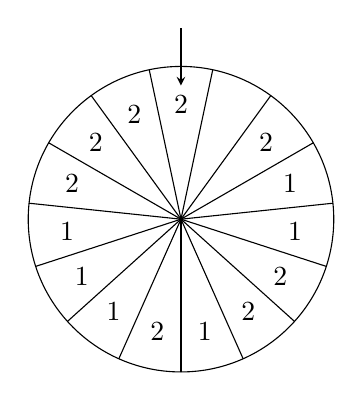
\begin{tikzpicture}[x=0.08\linewidth,y=0.08\linewidth, baseline={(T.base)}]
\draw (0,0) circle (2);
\draw[->,>=stealth] (0,2.5)node[below = 12pt](T){~} --(0,1.75);
\foreach \a/\n in {1/2,2/~,3/2,4/1,5/1,6/2,7/2,8/1,9/2,10/1,11/1,12/1,13/2,14/2,15/2}
{\draw(0,0)--(102-\a*24:2);
\node at (114-\a*24:1.5) {\n};}
\end{tikzpicture}\hfill~

\begin{tabularx}{\linewidth}{|*{4}{>{\centering \arraybackslash} X|}}\hline
Oui, en écrivant le nombre 1&
Oui, en écrivant le nombre 2&
Ce n'est pas possible&
Oui, en laissant le secteur vide\\ \hline
\end{tabularx}

\item On considère la liste de nombres suivante : \quad $5~;~1~;~3~;~10~;~17~;~11~;~10$.

Pour cette liste de nombres, que représente le nombre 5 ?

\begin{tabularx}{\linewidth}{|*{4}{>{\centering \arraybackslash} X|}}\hline
		La médiane & L'étendue & La moyenne & Rien de particulier\\ \hline
\end{tabularx}

\item Léa achète un vélo électrique. Pour le réserver, elle paye $\dfrac{1}{5}$ du prix au magasin. Le magasin lui propose de payer le reste en trois paiements d'un même montant.

Quelle fraction du prix du vélo représente l'un de ces trois paiements ?

%\begin{tabularx}{\linewidth}{|*{4}{>{\centering \arraybackslash} X|}}\hline
%$\dfrac{12}{5}$ & $\dfrac{1}{15}$ & $\dfrac{4}{15}$ & $\dfrac{3}{5}$ \\		\hline
%\end{tabularx}

\begin{tblr}{hlines, vlines, colspec={*{4}{X[c]}}}
$\dfrac{12}{5}$ & $\dfrac{1}{15}$ & $\dfrac{4}{15}$ & $\dfrac{3}{5}$ \\
\end{tblr}
\end{enumerate}


